\documentclass[twoside]{book}

% Packages required by doxygen
\usepackage{fixltx2e}
\usepackage{calc}
\usepackage{doxygen}
\usepackage[export]{adjustbox} % also loads graphicx
\usepackage{graphicx}
\usepackage[utf8]{inputenc}
\usepackage{makeidx}
\usepackage{multicol}
\usepackage{multirow}
\PassOptionsToPackage{warn}{textcomp}
\usepackage{textcomp}
\usepackage[nointegrals]{wasysym}
\usepackage[table]{xcolor}

% Font selection
\usepackage[T1]{fontenc}
\usepackage[scaled=.90]{helvet}
\usepackage{courier}
\usepackage{amssymb}
\usepackage{sectsty}
\renewcommand{\familydefault}{\sfdefault}
\allsectionsfont{%
  \fontseries{bc}\selectfont%
  \color{darkgray}%
}
\renewcommand{\DoxyLabelFont}{%
  \fontseries{bc}\selectfont%
  \color{darkgray}%
}
\newcommand{\+}{\discretionary{\mbox{\scriptsize$\hookleftarrow$}}{}{}}

% Page & text layout
\usepackage{geometry}
\geometry{%
  a4paper,%
  top=2.5cm,%
  bottom=2.5cm,%
  left=2.5cm,%
  right=2.5cm%
}
\tolerance=750
\hfuzz=15pt
\hbadness=750
\setlength{\emergencystretch}{15pt}
\setlength{\parindent}{0cm}
\setlength{\parskip}{3ex plus 2ex minus 2ex}
\makeatletter
\renewcommand{\paragraph}{%
  \@startsection{paragraph}{4}{0ex}{-1.0ex}{1.0ex}{%
    \normalfont\normalsize\bfseries\SS@parafont%
  }%
}
\renewcommand{\subparagraph}{%
  \@startsection{subparagraph}{5}{0ex}{-1.0ex}{1.0ex}{%
    \normalfont\normalsize\bfseries\SS@subparafont%
  }%
}
\makeatother

% Headers & footers
\usepackage{fancyhdr}
\pagestyle{fancyplain}
\fancyhead[LE]{\fancyplain{}{\bfseries\thepage}}
\fancyhead[CE]{\fancyplain{}{}}
\fancyhead[RE]{\fancyplain{}{\bfseries\leftmark}}
\fancyhead[LO]{\fancyplain{}{\bfseries\rightmark}}
\fancyhead[CO]{\fancyplain{}{}}
\fancyhead[RO]{\fancyplain{}{\bfseries\thepage}}
\fancyfoot[LE]{\fancyplain{}{}}
\fancyfoot[CE]{\fancyplain{}{}}
\fancyfoot[RE]{\fancyplain{}{\bfseries\scriptsize Generated by Doxygen }}
\fancyfoot[LO]{\fancyplain{}{\bfseries\scriptsize Generated by Doxygen }}
\fancyfoot[CO]{\fancyplain{}{}}
\fancyfoot[RO]{\fancyplain{}{}}
\renewcommand{\footrulewidth}{0.4pt}
\renewcommand{\chaptermark}[1]{%
  \markboth{#1}{}%
}
\renewcommand{\sectionmark}[1]{%
  \markright{\thesection\ #1}%
}

% Indices & bibliography
\usepackage{natbib}
\usepackage[titles]{tocloft}
\setcounter{tocdepth}{3}
\setcounter{secnumdepth}{5}
\makeindex

% Hyperlinks (required, but should be loaded last)
\usepackage{ifpdf}
\ifpdf
  \usepackage[pdftex,pagebackref=true]{hyperref}
\else
  \usepackage[ps2pdf,pagebackref=true]{hyperref}
\fi
\hypersetup{%
  colorlinks=true,%
  linkcolor=blue,%
  citecolor=blue,%
  unicode%
}

% Custom commands
\newcommand{\clearemptydoublepage}{%
  \newpage{\pagestyle{empty}\cleardoublepage}%
}

\usepackage{caption}
\captionsetup{labelsep=space,justification=centering,font={bf},singlelinecheck=off,skip=4pt,position=top}

%===== C O N T E N T S =====

\begin{document}

% Titlepage & ToC
\hypersetup{pageanchor=false,
             bookmarksnumbered=true,
             pdfencoding=unicode
            }
\pagenumbering{alph}
\begin{titlepage}
\vspace*{7cm}
\begin{center}%
{\Large sorkin\+Ryan\+A1 }\\
\vspace*{1cm}
{\large Generated by Doxygen 1.8.13}\\
\end{center}
\end{titlepage}
\clearemptydoublepage
\pagenumbering{roman}
\tableofcontents
\clearemptydoublepage
\pagenumbering{arabic}
\hypersetup{pageanchor=true}

%--- Begin generated contents ---
\chapter{Class Index}
\section{Class List}
Here are the classes, structs, unions and interfaces with brief descriptions\+:\begin{DoxyCompactList}
\item\contentsline{section}{\hyperlink{structcar}{car} }{\pageref{structcar}}{}
\item\contentsline{section}{\hyperlink{structQueue}{Queue} }{\pageref{structQueue}}{}
\end{DoxyCompactList}

\chapter{File Index}
\section{File List}
Here is a list of all documented files with brief descriptions\+:\begin{DoxyCompactList}
\item\contentsline{section}{include/\hyperlink{queueAPI_8h}{queue\+A\+P\+I.\+h} \\*File containing the function definitions of a queue }{\pageref{queueAPI_8h}}{}
\item\contentsline{section}{include/\hyperlink{sorkinRyanA1Libray_8h}{sorkin\+Ryan\+A1\+Libray.\+h} \\*File containing the functions to be used in assignment 1 that are not to be used in either list or queue A\+DT. Also includes car struct }{\pageref{sorkinRyanA1Libray_8h}}{}
\end{DoxyCompactList}

\chapter{Class Documentation}
\hypertarget{structcar}{}\section{car Struct Reference}
\label{structcar}\index{car@{car}}


{\ttfamily \#include $<$sorkin\+Ryan\+A1\+Libray.\+h$>$}

\subsection*{Public Attributes}
\begin{DoxyCompactItemize}
\item 
char \hyperlink{structcar_a4208701f83f56a82b4c60497ffca2932}{coming\+From} \mbox{[}2\mbox{]}
\item 
char \hyperlink{structcar_a38d24547773184258c1f98335a440e1c}{direction} \mbox{[}2\mbox{]}
\item 
float \hyperlink{structcar_ab23c46d7acda96f787f99e9930d1b1b6}{arrival\+Time}
\item 
float \hyperlink{structcar_a166a1d2ea40ef5977d26c3761a2a39c8}{wait\+Time}
\item 
float \hyperlink{structcar_a75e54f35b43292e1e2a30e54627d20ea}{travel\+Time}
\end{DoxyCompactItemize}


\subsection{Detailed Description}
Car struct that is meant to go inside the queue for the assignment simulation 

\subsection{Member Data Documentation}
\mbox{\Hypertarget{structcar_ab23c46d7acda96f787f99e9930d1b1b6}\label{structcar_ab23c46d7acda96f787f99e9930d1b1b6}} 
\index{car@{car}!arrival\+Time@{arrival\+Time}}
\index{arrival\+Time@{arrival\+Time}!car@{car}}
\subsubsection{\texorpdfstring{arrival\+Time}{arrivalTime}}
{\footnotesize\ttfamily float car\+::arrival\+Time}

Direction car is going (F, R, L) \mbox{\Hypertarget{structcar_a4208701f83f56a82b4c60497ffca2932}\label{structcar_a4208701f83f56a82b4c60497ffca2932}} 
\index{car@{car}!coming\+From@{coming\+From}}
\index{coming\+From@{coming\+From}!car@{car}}
\subsubsection{\texorpdfstring{coming\+From}{comingFrom}}
{\footnotesize\ttfamily char car\+::coming\+From\mbox{[}2\mbox{]}}

Direction car is coming from (N, E, S, W) \mbox{\Hypertarget{structcar_a38d24547773184258c1f98335a440e1c}\label{structcar_a38d24547773184258c1f98335a440e1c}} 
\index{car@{car}!direction@{direction}}
\index{direction@{direction}!car@{car}}
\subsubsection{\texorpdfstring{direction}{direction}}
{\footnotesize\ttfamily char car\+::direction\mbox{[}2\mbox{]}}

Direction car is coming from (N, E, S, W) \mbox{\Hypertarget{structcar_a75e54f35b43292e1e2a30e54627d20ea}\label{structcar_a75e54f35b43292e1e2a30e54627d20ea}} 
\index{car@{car}!travel\+Time@{travel\+Time}}
\index{travel\+Time@{travel\+Time}!car@{car}}
\subsubsection{\texorpdfstring{travel\+Time}{travelTime}}
{\footnotesize\ttfamily float car\+::travel\+Time}

How long the car is waiting at the front of its line \mbox{\Hypertarget{structcar_a166a1d2ea40ef5977d26c3761a2a39c8}\label{structcar_a166a1d2ea40ef5977d26c3761a2a39c8}} 
\index{car@{car}!wait\+Time@{wait\+Time}}
\index{wait\+Time@{wait\+Time}!car@{car}}
\subsubsection{\texorpdfstring{wait\+Time}{waitTime}}
{\footnotesize\ttfamily float car\+::wait\+Time}

Time the car arrived in the queue 

The documentation for this struct was generated from the following file\+:\begin{DoxyCompactItemize}
\item 
include/\hyperlink{sorkinRyanA1Libray_8h}{sorkin\+Ryan\+A1\+Libray.\+h}\end{DoxyCompactItemize}

\hypertarget{structQueue}{}\section{Queue Struct Reference}
\label{structQueue}\index{Queue@{Queue}}


{\ttfamily \#include $<$queue\+A\+P\+I.\+h$>$}

\subsection*{Public Attributes}
\begin{DoxyCompactItemize}
\item 
List $\ast$ \hyperlink{structQueue_a10b93f38cf61fc10d4bd49942eb475f1}{the\+List}
\item 
Node $\ast$ \hyperlink{structQueue_a36ab375d24d41bcc1d598c132700835b}{front}
\item 
Node $\ast$ \hyperlink{structQueue_aaf188b8da9524a67e909f14d78563dab}{back}
\item 
int \hyperlink{structQueue_a72159731344d08720fbb96bc482b9c10}{length}
\end{DoxyCompactItemize}


\subsection{Detailed Description}
A struct for the \hyperlink{structQueue}{Queue} A\+DT 

\subsection{Member Data Documentation}
\mbox{\Hypertarget{structQueue_aaf188b8da9524a67e909f14d78563dab}\label{structQueue_aaf188b8da9524a67e909f14d78563dab}} 
\index{Queue@{Queue}!back@{back}}
\index{back@{back}!Queue@{Queue}}
\subsubsection{\texorpdfstring{back}{back}}
{\footnotesize\ttfamily Node$\ast$ Queue\+::back}

Last node in the queue \mbox{\Hypertarget{structQueue_a36ab375d24d41bcc1d598c132700835b}\label{structQueue_a36ab375d24d41bcc1d598c132700835b}} 
\index{Queue@{Queue}!front@{front}}
\index{front@{front}!Queue@{Queue}}
\subsubsection{\texorpdfstring{front}{front}}
{\footnotesize\ttfamily Node$\ast$ Queue\+::front}

First node in the queue \mbox{\Hypertarget{structQueue_a72159731344d08720fbb96bc482b9c10}\label{structQueue_a72159731344d08720fbb96bc482b9c10}} 
\index{Queue@{Queue}!length@{length}}
\index{length@{length}!Queue@{Queue}}
\subsubsection{\texorpdfstring{length}{length}}
{\footnotesize\ttfamily int Queue\+::length}

length of the queue \mbox{\Hypertarget{structQueue_a10b93f38cf61fc10d4bd49942eb475f1}\label{structQueue_a10b93f38cf61fc10d4bd49942eb475f1}} 
\index{Queue@{Queue}!the\+List@{the\+List}}
\index{the\+List@{the\+List}!Queue@{Queue}}
\subsubsection{\texorpdfstring{the\+List}{theList}}
{\footnotesize\ttfamily List$\ast$ Queue\+::the\+List}

A List to be stored inside the queue 

The documentation for this struct was generated from the following file\+:\begin{DoxyCompactItemize}
\item 
include/\hyperlink{queueAPI_8h}{queue\+A\+P\+I.\+h}\end{DoxyCompactItemize}

\chapter{File Documentation}
\hypertarget{queueAPI_8h}{}\section{include/queue\+A\+PI.h File Reference}
\label{queueAPI_8h}\index{include/queue\+A\+P\+I.\+h@{include/queue\+A\+P\+I.\+h}}


File containing the function definitions of a queue.  


{\ttfamily \#include $<$stdio.\+h$>$}\newline
{\ttfamily \#include $<$stdlib.\+h$>$}\newline
{\ttfamily \#include \char`\"{}Linked\+List\+A\+P\+I.\+h\char`\"{}}\newline
Include dependency graph for queue\+A\+P\+I.\+h\+:\nopagebreak
\begin{figure}[H]
\begin{center}
\leavevmode
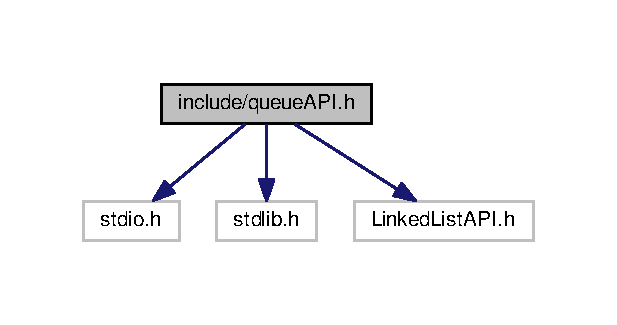
\includegraphics[width=296pt]{queueAPI_8h__incl}
\end{center}
\end{figure}
This graph shows which files directly or indirectly include this file\+:\nopagebreak
\begin{figure}[H]
\begin{center}
\leavevmode
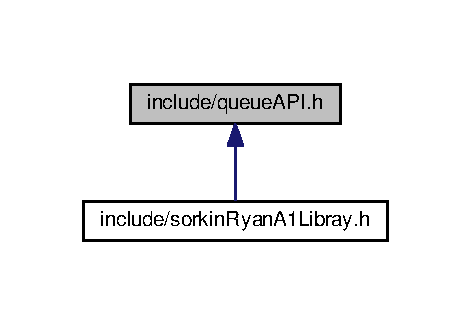
\includegraphics[width=226pt]{queueAPI_8h__dep__incl}
\end{center}
\end{figure}
\subsection*{Classes}
\begin{DoxyCompactItemize}
\item 
struct \hyperlink{structQueue}{Queue}
\end{DoxyCompactItemize}
\subsection*{Typedefs}
\begin{DoxyCompactItemize}
\item 
typedef struct \hyperlink{structQueue}{Queue} \hyperlink{queueAPI_8h_ad4f29a362a072ba563b41ae8e935c6fc}{Queue}
\end{DoxyCompactItemize}
\subsection*{Functions}
\begin{DoxyCompactItemize}
\item 
\hyperlink{structQueue}{Queue} $\ast$ \hyperlink{queueAPI_8h_ac40478244e5c37e8dca06fa3e3b7c6fe}{create} (List $\ast$list)
\item 
void \hyperlink{queueAPI_8h_ab140f2bb51a79ba1e396a3346db0ef06}{destroy} (\hyperlink{structQueue}{Queue} $\ast$queue)
\item 
void \hyperlink{queueAPI_8h_a2880857fd76132b3402354ea78dff7ff}{add} (\hyperlink{structQueue}{Queue} $\ast$queue, void $\ast$data)
\item 
void $\ast$ \hyperlink{queueAPI_8h_a0133c7e4da948f6a9368a0b0c4e2fbf9}{dequeue} (\hyperlink{structQueue}{Queue} $\ast$queue)
\item 
int \hyperlink{queueAPI_8h_a2a0de0f79d046b25877028a89858f843}{length} (\hyperlink{structQueue}{Queue} $\ast$queue)
\item 
int \hyperlink{queueAPI_8h_ae2701ab012e9ff60a04d6ffd07a42e1b}{is\+Empty} (\hyperlink{structQueue}{Queue} $\ast$queue)
\end{DoxyCompactItemize}


\subsection{Detailed Description}
File containing the function definitions of a queue. 

\begin{DoxyAuthor}{Author}
Ryan Sorkin 
\end{DoxyAuthor}
\begin{DoxyDate}{Date}
May 2018 
\end{DoxyDate}


\subsection{Typedef Documentation}
\mbox{\Hypertarget{queueAPI_8h_ad4f29a362a072ba563b41ae8e935c6fc}\label{queueAPI_8h_ad4f29a362a072ba563b41ae8e935c6fc}} 
\index{queue\+A\+P\+I.\+h@{queue\+A\+P\+I.\+h}!Queue@{Queue}}
\index{Queue@{Queue}!queue\+A\+P\+I.\+h@{queue\+A\+P\+I.\+h}}
\subsubsection{\texorpdfstring{Queue}{Queue}}
{\footnotesize\ttfamily typedef struct \hyperlink{structQueue}{Queue} \hyperlink{structQueue}{Queue}}

A struct for the \hyperlink{structQueue}{Queue} A\+DT 

\subsection{Function Documentation}
\mbox{\Hypertarget{queueAPI_8h_a2880857fd76132b3402354ea78dff7ff}\label{queueAPI_8h_a2880857fd76132b3402354ea78dff7ff}} 
\index{queue\+A\+P\+I.\+h@{queue\+A\+P\+I.\+h}!add@{add}}
\index{add@{add}!queue\+A\+P\+I.\+h@{queue\+A\+P\+I.\+h}}
\subsubsection{\texorpdfstring{add()}{add()}}
{\footnotesize\ttfamily void add (\begin{DoxyParamCaption}\item[{\hyperlink{structQueue}{Queue} $\ast$}]{queue,  }\item[{void $\ast$}]{data }\end{DoxyParamCaption})}

Function to add a pointer to any data to the queue Adds data to the end of the queue 
\begin{DoxyParams}{Parameters}
{\em queue} & A\+DT with memory allocated to it \\
\hline
{\em data} & to a void pointer to data that is non N\+U\+LL \\
\hline
\end{DoxyParams}
\mbox{\Hypertarget{queueAPI_8h_ac40478244e5c37e8dca06fa3e3b7c6fe}\label{queueAPI_8h_ac40478244e5c37e8dca06fa3e3b7c6fe}} 
\index{queue\+A\+P\+I.\+h@{queue\+A\+P\+I.\+h}!create@{create}}
\index{create@{create}!queue\+A\+P\+I.\+h@{queue\+A\+P\+I.\+h}}
\subsubsection{\texorpdfstring{create()}{create()}}
{\footnotesize\ttfamily \hyperlink{structQueue}{Queue}$\ast$ create (\begin{DoxyParamCaption}\item[{List $\ast$}]{list }\end{DoxyParamCaption})}

Function to allocate memory and return a queue A\+DT that will encapsulate a list A\+DT \begin{DoxyReturn}{Returns}
pointer to the \hyperlink{structQueue}{Queue} which has memory allocated to it 
\end{DoxyReturn}

\begin{DoxyParams}{Parameters}
{\em list} & struct that has the contents of the queue \\
\hline
\end{DoxyParams}
\mbox{\Hypertarget{queueAPI_8h_a0133c7e4da948f6a9368a0b0c4e2fbf9}\label{queueAPI_8h_a0133c7e4da948f6a9368a0b0c4e2fbf9}} 
\index{queue\+A\+P\+I.\+h@{queue\+A\+P\+I.\+h}!dequeue@{dequeue}}
\index{dequeue@{dequeue}!queue\+A\+P\+I.\+h@{queue\+A\+P\+I.\+h}}
\subsubsection{\texorpdfstring{dequeue()}{dequeue()}}
{\footnotesize\ttfamily void$\ast$ dequeue (\begin{DoxyParamCaption}\item[{\hyperlink{structQueue}{Queue} $\ast$}]{queue }\end{DoxyParamCaption})}

Removes the front item in the \hyperlink{structQueue}{Queue} and returns it 
\begin{DoxyParams}{Parameters}
{\em queue} & A\+DT with memory allocated to it \\
\hline
\end{DoxyParams}
\begin{DoxyReturn}{Returns}
A void pointer to data from the front of the queue 
\end{DoxyReturn}
\mbox{\Hypertarget{queueAPI_8h_ab140f2bb51a79ba1e396a3346db0ef06}\label{queueAPI_8h_ab140f2bb51a79ba1e396a3346db0ef06}} 
\index{queue\+A\+P\+I.\+h@{queue\+A\+P\+I.\+h}!destroy@{destroy}}
\index{destroy@{destroy}!queue\+A\+P\+I.\+h@{queue\+A\+P\+I.\+h}}
\subsubsection{\texorpdfstring{destroy()}{destroy()}}
{\footnotesize\ttfamily void destroy (\begin{DoxyParamCaption}\item[{\hyperlink{structQueue}{Queue} $\ast$}]{queue }\end{DoxyParamCaption})}

Function to destroy and free all memory allocated for the \hyperlink{structQueue}{Queue} 
\begin{DoxyParams}{Parameters}
{\em queue} & A\+DT with memory allocated to it \\
\hline
\end{DoxyParams}
\mbox{\Hypertarget{queueAPI_8h_ae2701ab012e9ff60a04d6ffd07a42e1b}\label{queueAPI_8h_ae2701ab012e9ff60a04d6ffd07a42e1b}} 
\index{queue\+A\+P\+I.\+h@{queue\+A\+P\+I.\+h}!is\+Empty@{is\+Empty}}
\index{is\+Empty@{is\+Empty}!queue\+A\+P\+I.\+h@{queue\+A\+P\+I.\+h}}
\subsubsection{\texorpdfstring{is\+Empty()}{isEmpty()}}
{\footnotesize\ttfamily int is\+Empty (\begin{DoxyParamCaption}\item[{\hyperlink{structQueue}{Queue} $\ast$}]{queue }\end{DoxyParamCaption})}

Function to determine if the queue is empty or not Returns 1 if list is null or empty, 0 otherwise 
\begin{DoxyParams}{Parameters}
{\em queue} & A\+DT with memory allocated to it \\
\hline
\end{DoxyParams}
\begin{DoxyReturn}{Returns}
An int to represent true or false 
\end{DoxyReturn}
\mbox{\Hypertarget{queueAPI_8h_a2a0de0f79d046b25877028a89858f843}\label{queueAPI_8h_a2a0de0f79d046b25877028a89858f843}} 
\index{queue\+A\+P\+I.\+h@{queue\+A\+P\+I.\+h}!length@{length}}
\index{length@{length}!queue\+A\+P\+I.\+h@{queue\+A\+P\+I.\+h}}
\subsubsection{\texorpdfstring{length()}{length()}}
{\footnotesize\ttfamily int length (\begin{DoxyParamCaption}\item[{\hyperlink{structQueue}{Queue} $\ast$}]{queue }\end{DoxyParamCaption})}

A function to determine the number of items in a queue 
\begin{DoxyParams}{Parameters}
{\em queue} & A\+DT with memory allocated to it \\
\hline
\end{DoxyParams}
\begin{DoxyReturn}{Returns}
Length of the queue as an int 
\end{DoxyReturn}

\hypertarget{sorkinRyanA1Libray_8h}{}\section{include/sorkin\+Ryan\+A1\+Libray.h File Reference}
\label{sorkinRyanA1Libray_8h}\index{include/sorkin\+Ryan\+A1\+Libray.\+h@{include/sorkin\+Ryan\+A1\+Libray.\+h}}


File containing the functions to be used in assignment 1 that are not to be used in either list or queue A\+DT. Also includes car struct.  


{\ttfamily \#include $<$stdio.\+h$>$}\newline
{\ttfamily \#include $<$stdlib.\+h$>$}\newline
{\ttfamily \#include \char`\"{}Linked\+List\+A\+P\+I.\+h\char`\"{}}\newline
{\ttfamily \#include \char`\"{}queue\+A\+P\+I.\+h\char`\"{}}\newline
Include dependency graph for sorkin\+Ryan\+A1\+Libray.\+h\+:\nopagebreak
\begin{figure}[H]
\begin{center}
\leavevmode
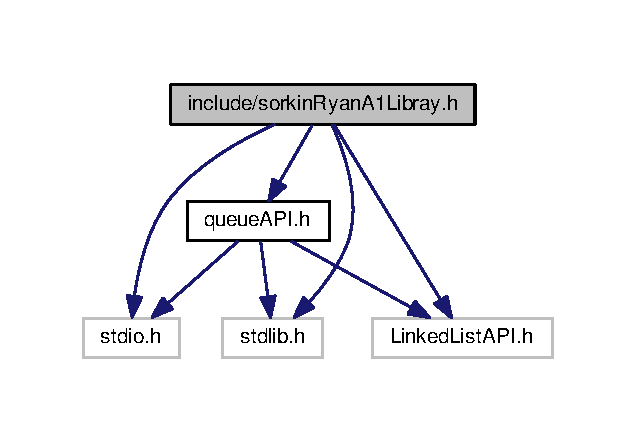
\includegraphics[width=305pt]{sorkinRyanA1Libray_8h__incl}
\end{center}
\end{figure}
\subsection*{Classes}
\begin{DoxyCompactItemize}
\item 
struct \hyperlink{structcar}{car}
\end{DoxyCompactItemize}
\subsection*{Typedefs}
\begin{DoxyCompactItemize}
\item 
typedef struct \hyperlink{structcar}{car} \hyperlink{sorkinRyanA1Libray_8h_a367f8f21caa33f1a5af286dfb673d34a}{Car}
\end{DoxyCompactItemize}
\subsection*{Functions}
\begin{DoxyCompactItemize}
\item 
void \hyperlink{sorkinRyanA1Libray_8h_a80c8f2163fcaedba3683bf1593cbc744}{print\+Car\+Data} (void $\ast$data)
\item 
int \hyperlink{sorkinRyanA1Libray_8h_a00f47305e5583254cb8fa41544525684}{compare\+Cars} (const void $\ast$first, const void $\ast$second)
\item 
void \hyperlink{sorkinRyanA1Libray_8h_a4528b0a7192141fc985f72a8c8e757c1}{delete\+Car} (void $\ast$data)
\item 
\hyperlink{sorkinRyanA1Libray_8h_a367f8f21caa33f1a5af286dfb673d34a}{Car} $\ast$ \hyperlink{sorkinRyanA1Libray_8h_a6590d516be6c90b9fccc4da7b62d9606}{make\+Car} (char $\ast$data)
\item 
Node $\ast$ \hyperlink{sorkinRyanA1Libray_8h_a02d9f8d6da079c2c86ed175b2f2f2e80}{get\+Turn} (\hyperlink{structQueue}{Queue} $\ast$north\+Queue, \hyperlink{structQueue}{Queue} $\ast$east\+Queue, \hyperlink{structQueue}{Queue} $\ast$south\+Queue, \hyperlink{structQueue}{Queue} $\ast$west\+Queue, float counter)
\item 
void \hyperlink{sorkinRyanA1Libray_8h_a710bbf461a8f8c8014172c6e88521687}{move\+Car} (\hyperlink{structQueue}{Queue} $\ast$north\+Queue, \hyperlink{structQueue}{Queue} $\ast$east\+Queue, \hyperlink{structQueue}{Queue} $\ast$south\+Queue, \hyperlink{structQueue}{Queue} $\ast$west\+Queue, Node $\ast$node, float $\ast$counter)
\item 
void \hyperlink{sorkinRyanA1Libray_8h_aa4f1ee86b74be5deb65422cb80788e9b}{wait\+Per\+Lane} (Node $\ast$node, float lanes\mbox{[}2\mbox{]}\mbox{[}4\mbox{]}, float counter)
\item 
void \hyperlink{sorkinRyanA1Libray_8h_a13cdb53bb7789345dced3e8358b06375}{print\+Stats} (float lanes\mbox{[}2\mbox{]}\mbox{[}4\mbox{]}, float counter, float max\+Wait, int car\+Counter)
\item 
void \hyperlink{sorkinRyanA1Libray_8h_abfd100616b7bb5f6fa926d5a5c8d0a37}{update\+Wait\+Time} (\hyperlink{structQueue}{Queue} $\ast$to\+Update, float counter, float travel\+Time)
\end{DoxyCompactItemize}


\subsection{Detailed Description}
File containing the functions to be used in assignment 1 that are not to be used in either list or queue A\+DT. Also includes car struct. 

\begin{DoxyAuthor}{Author}
Ryan Sorkin 
\end{DoxyAuthor}
\begin{DoxyDate}{Date}
June 2018 
\end{DoxyDate}


\subsection{Typedef Documentation}
\mbox{\Hypertarget{sorkinRyanA1Libray_8h_a367f8f21caa33f1a5af286dfb673d34a}\label{sorkinRyanA1Libray_8h_a367f8f21caa33f1a5af286dfb673d34a}} 
\index{sorkin\+Ryan\+A1\+Libray.\+h@{sorkin\+Ryan\+A1\+Libray.\+h}!Car@{Car}}
\index{Car@{Car}!sorkin\+Ryan\+A1\+Libray.\+h@{sorkin\+Ryan\+A1\+Libray.\+h}}
\subsubsection{\texorpdfstring{Car}{Car}}
{\footnotesize\ttfamily typedef struct \hyperlink{structcar}{car}  \hyperlink{sorkinRyanA1Libray_8h_a367f8f21caa33f1a5af286dfb673d34a}{Car}}

Car struct that is meant to go inside the queue for the assignment simulation 

\subsection{Function Documentation}
\mbox{\Hypertarget{sorkinRyanA1Libray_8h_a00f47305e5583254cb8fa41544525684}\label{sorkinRyanA1Libray_8h_a00f47305e5583254cb8fa41544525684}} 
\index{sorkin\+Ryan\+A1\+Libray.\+h@{sorkin\+Ryan\+A1\+Libray.\+h}!compare\+Cars@{compare\+Cars}}
\index{compare\+Cars@{compare\+Cars}!sorkin\+Ryan\+A1\+Libray.\+h@{sorkin\+Ryan\+A1\+Libray.\+h}}
\subsubsection{\texorpdfstring{compare\+Cars()}{compareCars()}}
{\footnotesize\ttfamily int compare\+Cars (\begin{DoxyParamCaption}\item[{const void $\ast$}]{first,  }\item[{const void $\ast$}]{second }\end{DoxyParamCaption})}

Compare the arrival time of two cars, return\+: 0 if they arrived at the same time 1 if car 1 arrived first -\/1 if car 1 arrived second 
\begin{DoxyParams}{Parameters}
{\em first} & void pointer to first car to be compared \\
\hline
{\em second} & void pointer to second car to be compared \\
\hline
\end{DoxyParams}
\mbox{\Hypertarget{sorkinRyanA1Libray_8h_a4528b0a7192141fc985f72a8c8e757c1}\label{sorkinRyanA1Libray_8h_a4528b0a7192141fc985f72a8c8e757c1}} 
\index{sorkin\+Ryan\+A1\+Libray.\+h@{sorkin\+Ryan\+A1\+Libray.\+h}!delete\+Car@{delete\+Car}}
\index{delete\+Car@{delete\+Car}!sorkin\+Ryan\+A1\+Libray.\+h@{sorkin\+Ryan\+A1\+Libray.\+h}}
\subsubsection{\texorpdfstring{delete\+Car()}{deleteCar()}}
{\footnotesize\ttfamily void delete\+Car (\begin{DoxyParamCaption}\item[{void $\ast$}]{data }\end{DoxyParamCaption})}

Free the memory associated with a car 
\begin{DoxyParams}{Parameters}
{\em data} & to a void pointer to Car$\ast$ to be freed \\
\hline
\end{DoxyParams}
\mbox{\Hypertarget{sorkinRyanA1Libray_8h_a02d9f8d6da079c2c86ed175b2f2f2e80}\label{sorkinRyanA1Libray_8h_a02d9f8d6da079c2c86ed175b2f2f2e80}} 
\index{sorkin\+Ryan\+A1\+Libray.\+h@{sorkin\+Ryan\+A1\+Libray.\+h}!get\+Turn@{get\+Turn}}
\index{get\+Turn@{get\+Turn}!sorkin\+Ryan\+A1\+Libray.\+h@{sorkin\+Ryan\+A1\+Libray.\+h}}
\subsubsection{\texorpdfstring{get\+Turn()}{getTurn()}}
{\footnotesize\ttfamily Node$\ast$ get\+Turn (\begin{DoxyParamCaption}\item[{\hyperlink{structQueue}{Queue} $\ast$}]{north\+Queue,  }\item[{\hyperlink{structQueue}{Queue} $\ast$}]{east\+Queue,  }\item[{\hyperlink{structQueue}{Queue} $\ast$}]{south\+Queue,  }\item[{\hyperlink{structQueue}{Queue} $\ast$}]{west\+Queue,  }\item[{float}]{counter }\end{DoxyParamCaption})}

Determines if the next car in the queue is ready to cross the intersection, depends on current time 
\begin{DoxyParams}{Parameters}
{\em north\+Queue} & the queue of cars coming from North \\
\hline
{\em east\+Queue} & the queue of cars coming from East \\
\hline
{\em south\+Queue} & the queue of cars coming from South \\
\hline
{\em west\+Queue} & the queue of cars coming from West \\
\hline
{\em counter} & is the current simulation time \\
\hline
\end{DoxyParams}
\begin{DoxyReturn}{Returns}
a pointer to the car whos turn it is 
\end{DoxyReturn}
\mbox{\Hypertarget{sorkinRyanA1Libray_8h_a6590d516be6c90b9fccc4da7b62d9606}\label{sorkinRyanA1Libray_8h_a6590d516be6c90b9fccc4da7b62d9606}} 
\index{sorkin\+Ryan\+A1\+Libray.\+h@{sorkin\+Ryan\+A1\+Libray.\+h}!make\+Car@{make\+Car}}
\index{make\+Car@{make\+Car}!sorkin\+Ryan\+A1\+Libray.\+h@{sorkin\+Ryan\+A1\+Libray.\+h}}
\subsubsection{\texorpdfstring{make\+Car()}{makeCar()}}
{\footnotesize\ttfamily \hyperlink{sorkinRyanA1Libray_8h_a367f8f21caa33f1a5af286dfb673d34a}{Car}$\ast$ make\+Car (\begin{DoxyParamCaption}\item[{char $\ast$}]{data }\end{DoxyParamCaption})}

Create and return a car based on info read from file 
\begin{DoxyParams}{Parameters}
{\em data} & pointer to string read in from file \\
\hline
\end{DoxyParams}
\begin{DoxyReturn}{Returns}
a pointer to allocated memory to a Car struct 
\end{DoxyReturn}
\mbox{\Hypertarget{sorkinRyanA1Libray_8h_a710bbf461a8f8c8014172c6e88521687}\label{sorkinRyanA1Libray_8h_a710bbf461a8f8c8014172c6e88521687}} 
\index{sorkin\+Ryan\+A1\+Libray.\+h@{sorkin\+Ryan\+A1\+Libray.\+h}!move\+Car@{move\+Car}}
\index{move\+Car@{move\+Car}!sorkin\+Ryan\+A1\+Libray.\+h@{sorkin\+Ryan\+A1\+Libray.\+h}}
\subsubsection{\texorpdfstring{move\+Car()}{moveCar()}}
{\footnotesize\ttfamily void move\+Car (\begin{DoxyParamCaption}\item[{\hyperlink{structQueue}{Queue} $\ast$}]{north\+Queue,  }\item[{\hyperlink{structQueue}{Queue} $\ast$}]{east\+Queue,  }\item[{\hyperlink{structQueue}{Queue} $\ast$}]{south\+Queue,  }\item[{\hyperlink{structQueue}{Queue} $\ast$}]{west\+Queue,  }\item[{Node $\ast$}]{node,  }\item[{float $\ast$}]{counter }\end{DoxyParamCaption})}

\char`\"{}\+Move\char`\"{} the car across the intersection and increase the simulation timer depending on the direction the car went 
\begin{DoxyParams}{Parameters}
{\em north\+Queue} & the queue of cars coming from North \\
\hline
{\em east\+Queue} & the queue of cars coming from East \\
\hline
{\em south\+Queue} & the queue of cars coming from South \\
\hline
{\em west\+Queue} & the queue of cars coming from West \\
\hline
{\em node} & that holds the current car going \\
\hline
{\em counter} & pointer of the simulation timer \\
\hline
\end{DoxyParams}
\mbox{\Hypertarget{sorkinRyanA1Libray_8h_a80c8f2163fcaedba3683bf1593cbc744}\label{sorkinRyanA1Libray_8h_a80c8f2163fcaedba3683bf1593cbc744}} 
\index{sorkin\+Ryan\+A1\+Libray.\+h@{sorkin\+Ryan\+A1\+Libray.\+h}!print\+Car\+Data@{print\+Car\+Data}}
\index{print\+Car\+Data@{print\+Car\+Data}!sorkin\+Ryan\+A1\+Libray.\+h@{sorkin\+Ryan\+A1\+Libray.\+h}}
\subsubsection{\texorpdfstring{print\+Car\+Data()}{printCarData()}}
{\footnotesize\ttfamily void print\+Car\+Data (\begin{DoxyParamCaption}\item[{void $\ast$}]{data }\end{DoxyParamCaption})}

Once a car is passed in its information is printed 
\begin{DoxyParams}{Parameters}
{\em data} & to a void pointer, expected to be a Car $\ast$ \\
\hline
\end{DoxyParams}
\mbox{\Hypertarget{sorkinRyanA1Libray_8h_a13cdb53bb7789345dced3e8358b06375}\label{sorkinRyanA1Libray_8h_a13cdb53bb7789345dced3e8358b06375}} 
\index{sorkin\+Ryan\+A1\+Libray.\+h@{sorkin\+Ryan\+A1\+Libray.\+h}!print\+Stats@{print\+Stats}}
\index{print\+Stats@{print\+Stats}!sorkin\+Ryan\+A1\+Libray.\+h@{sorkin\+Ryan\+A1\+Libray.\+h}}
\subsubsection{\texorpdfstring{print\+Stats()}{printStats()}}
{\footnotesize\ttfamily void print\+Stats (\begin{DoxyParamCaption}\item[{float}]{lanes\mbox{[}2\mbox{]}\mbox{[}4\mbox{]},  }\item[{float}]{counter,  }\item[{float}]{max\+Wait,  }\item[{int}]{car\+Counter }\end{DoxyParamCaption})}

Display stats regarding the simulation\+: Total time, longest wait, ave wait, ave wait per lane 
\begin{DoxyParams}{Parameters}
{\em lanes} & that stores a 2D array to keep track of total travel time, cars traveled per lane \\
\hline
{\em counter} & to the simulation time \\
\hline
{\em max\+Wait} & is the longest wait time so far \\
\hline
{\em car\+Counter} & is the number of cars that have travelled through the simulation \\
\hline
\end{DoxyParams}
\mbox{\Hypertarget{sorkinRyanA1Libray_8h_abfd100616b7bb5f6fa926d5a5c8d0a37}\label{sorkinRyanA1Libray_8h_abfd100616b7bb5f6fa926d5a5c8d0a37}} 
\index{sorkin\+Ryan\+A1\+Libray.\+h@{sorkin\+Ryan\+A1\+Libray.\+h}!update\+Wait\+Time@{update\+Wait\+Time}}
\index{update\+Wait\+Time@{update\+Wait\+Time}!sorkin\+Ryan\+A1\+Libray.\+h@{sorkin\+Ryan\+A1\+Libray.\+h}}
\subsubsection{\texorpdfstring{update\+Wait\+Time()}{updateWaitTime()}}
{\footnotesize\ttfamily void update\+Wait\+Time (\begin{DoxyParamCaption}\item[{\hyperlink{structQueue}{Queue} $\ast$}]{to\+Update,  }\item[{float}]{counter,  }\item[{float}]{travel\+Time }\end{DoxyParamCaption})}

Updates the time that those at the front of each lane have waited for their turn 
\begin{DoxyParams}{Parameters}
{\em to\+Update} & is the \hyperlink{structQueue}{Queue} that needs to be updated \\
\hline
{\em counter} & to the simulation time \\
\hline
{\em travel\+Time} & how long the car going across the intersection takes to travel \\
\hline
\end{DoxyParams}
\mbox{\Hypertarget{sorkinRyanA1Libray_8h_aa4f1ee86b74be5deb65422cb80788e9b}\label{sorkinRyanA1Libray_8h_aa4f1ee86b74be5deb65422cb80788e9b}} 
\index{sorkin\+Ryan\+A1\+Libray.\+h@{sorkin\+Ryan\+A1\+Libray.\+h}!wait\+Per\+Lane@{wait\+Per\+Lane}}
\index{wait\+Per\+Lane@{wait\+Per\+Lane}!sorkin\+Ryan\+A1\+Libray.\+h@{sorkin\+Ryan\+A1\+Libray.\+h}}
\subsubsection{\texorpdfstring{wait\+Per\+Lane()}{waitPerLane()}}
{\footnotesize\ttfamily void wait\+Per\+Lane (\begin{DoxyParamCaption}\item[{Node $\ast$}]{node,  }\item[{float}]{lanes\mbox{[}2\mbox{]}\mbox{[}4\mbox{]},  }\item[{float}]{counter }\end{DoxyParamCaption})}

Keeps track of total wait time per lane and cars traveled per lane 
\begin{DoxyParams}{Parameters}
{\em node} & that stores the current car that is going across the intersection \\
\hline
{\em lanes} & that stores a 2D array to keep track of total travel time, cars traveled per lane \\
\hline
{\em counter} & to a simulation timer, to calculate wait time \\
\hline
\end{DoxyParams}

%--- End generated contents ---

% Index
\backmatter
\newpage
\phantomsection
\clearemptydoublepage
\addcontentsline{toc}{chapter}{Index}
\printindex

\end{document}
